\documentclass[12pt, a4paper]{report}
\usepackage{graphicx, array, amsthm, amssymb, amsmath, algorithm, algpseudocode, float, xcolor, thmtools, thmbox}
\usepackage[english]{babel}

\makeatletter
\renewcommand\thmbox@headstyle[2]{\bfseries #1}
\makeatother
\newtheorem[style=M,bodystyle=\normalfont]{theorem}{Theorem}
\newtheorem[style=M,bodystyle=\normalfont]{corollary}{Corollary}
\newtheorem[style=M,bodystyle=\normalfont]{lemma}{Lemma}
\newtheorem[style=M,bodystyle=\normalfont]{definition}{Definition}


\title{Foundation Of Operations Research \\ \textit{Theory}}
\author{Christian Rossi}
\date{Academic Year 2023-2024}

\begin{document}

\maketitle

\newpage

\begin{abstract}
    Operations Research is the branch of applied mathematics dealing with quantitative methods to analyze and solve
    complex real-world decision-making problems. 
    
    The course covers some fundamental concepts and methods of Operations Research pertaining to graph optimization, 
    linear programming and integer linear programming. 
    
    The emphasis is on optimization models and efficient algorithms with a wide range of important applications in 
    engineering and management.  
\end{abstract}

\newpage

\tableofcontents

\newpage
 
\chapter{Introduction}
    \section{Definition}
    \begin{definition}
        \emph{Operations Research} is the branch of mathematics in which mathematical models and quantitative methods are used to analyze complex decision-making problems and find
        near-optimal solutions.
    \end{definition}
    It is an interdisciplinary field at the interface of applied mathematics, computer science, economics and industrial engineering. 

    \section{Decision-making problems}
    \begin{definition}
        The \emph{decision-making problems} are problems in which we must choose a feasible solution among many alternatives based on one or several criteria. 
    \end{definition}
    The more complex decision-making problems are tackled via a mathematical modelling approach. 
    Those problems can be classified in the following categories: 
    \begin{enumerate}
        \item Assignment problem: given $m$ jobs and $m$ machines, suppose that each job can be executed by any machine and that $t_{ij}$ is the execution time of job $J_i$ one
            machine $M_j$. We want to decide which job assign to each machine to minimize the total execution time. Each job must be assigned to exactly one machine, and each 
            machine to exactly one job. The number of feasible solution is equal to $m!$. 
        \item Network design: we want to decide how to connect $n$ cities via a collection of possible links to minimize the total link cost. 
            Given a graph $G=(N,E)$ with a node $i \in N$ for each city and an edge $\{i,j\} \in E$ of cost $c_ij$, select a subset of edges of minimum total cost, guaranteeing that 
            all pairs of nodes are connected. The number of feasible solution is equal to $2^{\left\lvert E \right\rvert}$. 
        \item Shortest path: given a direct graph that represents a road network with distances (traveling times) for each arc, determine the shortest path between two points (nodes).
        \item Personnel scheduling: determine the week schedule for the hospital personnel, to minimize the number of people involved while meeting the daily requirements.
        \item Service management: determine how many desks to open at a given time of the day so that the average customer waiting time does not exceed a certain value. 
        \item Multi-criteria problem: decide which laptop to buy considering the price, the weight and the performance. 
        \item Maximum clique (community detection in social networks): determine the complete sub-graph of a graph, with the maximum number of vertices.
    \end{enumerate}

    \section{History}
    In the World War II, teams of scientists were asked to do research on the most efficient way to conduct the operations.
    In the decades after the war, the techniques became public and began to be applied more widely to problems in business, industry and society.
    During the industrial boom, the substantial increase in the size of the companies and organizations gave rise to more complex decision-making problems. 
    The favorable circumstances that permitted this were: 
    \begin{itemize}
        \item Fast progress in Operations Research and in numerical analysis methodologies. 
        \item Advent and diffusion of computers (more computing power and widespread software).
    \end{itemize}

    \section{Operations Research workflow}
    \begin{figure}[H]
        \centering
        
\includegraphics[width=1\linewidth]{images/study.png}
    \end{figure}
    The main steps in studying an Operations Research problem are: 
    \begin{enumerate}
        \item Define the problem.
        \item Build the model.
        \item Select or develop an appropriate algorithm. 
        \item Implement it or use an existing program. 
    \end{enumerate}
    After all this process we need to analyze the results with feedbacks (and eventually modify some previous step). 

    The model obtained with this process is a simplified representation of a real-world problem. To define it we must identify the fundamental elements of the problem and the main
    relationships among them. 
    \begin{example}
        A company produces three types of electronic devices: $D_1,D_2,D_3$, going through three main phases of the production process: assembly, refinement and quality control.
        The time required for each phase and product is: 
        \begin{table}[H]
            \centering
            \begin{tabular}{c|ccc|}
            \cline{2-4}
            \textbf{}                             & \textbf{$D_1$} & \textbf{$D_2$} & $D_3$ \\ \hline
            \multicolumn{1}{|c|}{Assembly}        & 80             & 70             & 120   \\
            \multicolumn{1}{|c|}{Refinement}      & 70             & 90             & 20    \\
            \multicolumn{1}{|c|}{Quality control} & 40             & 30             & 20    \\ \hline
            \end{tabular}
        \end{table}
        The available resources within the planning horizon in minutes are: 
        \begin{table}[H]
            \centering
            \begin{tabular}{|c|c|c|}
            \hline
            \textbf{Assembly} & \textbf{Refinement} & \textbf{Quality control} \\ \hline
            30 000            & 25 000              & 18 000                   \\ \hline
            \end{tabular}
        \end{table}
        The unary product for each product in: 
        \begin{table}[H]
            \centering
            \begin{tabular}{|c|c|c|}
            \hline
            $D_1$          & $D_2$          & $D_3$ \\ \hline
            1600           & 1000           & 2000  \\ \hline
            \end{tabular}
        \end{table}
        The main assumption is that the company can sell whatever it produces. 

        The mathematical model that describes the problem given before is the following: 
        \begin{itemize}
            \item Decision variables: $x_j$ is the number of devices $D_j$ produced for $j=1,2,3$.
            \item Objective function: we need to maximize the earning, so we have: 
                \[\max{z}=1.6x_1+1x_2+2x_3\]
            \item Constraints: they are on the production limit of each phase, that are: 
                \[80x_1+70x_2+120x_3 \leq 30000\]
                \[70x_1+90x_2+20x_3 \leq 25000\]
                \[40x_1+30x_2+20x_3 \leq 18000\]
            \item Variable type: the variables must be non-negative values, so we have $x_1,x_2,x_3 \geq 0$.
        \end{itemize}
    \end{example}
    \begin{example}
        An insurance company must decide which investments to select out of a given set of possible assets.
        \begin{table}[H]
            \centering
            \begin{tabular}{|c|ccc|}
            \hline
            \textbf{Investments} & \textbf{Area} & \textbf{Capital ($c_j$)} & \textbf{Return ($r_j$)} \\ \hline
            A (automotive)       & Germany       & $150 000$                & $11\%$                  \\
            B (automotive)       & Italy         & $150 000$                & $9\%$                   \\
            C (ICT)              & USA           & $60 000$                 & $13\%$                  \\
            D (ICT)              & Italy         & $100 000$                & $10\%$                  \\
            E (real estate)      & Italy         & $125 000$                & $8\%$                   \\
            F (real estate)      & France        & $100 000$                & $7\%$                   \\
            G (treasury bonds)   & Italy         & $50 000$                 & $3\%$                   \\
            H (treasury bonds)   & UK            & $80 000$                 & $5\%$                   \\ \hline
            \end{tabular}
        \end{table}
        The available capital is $600\:000$ euro. It is required to take at most five different investments. It is also required to take at maximum three investments in Italy and 
        maximum three abroad. 

        The mathematical model that describes the problem given before is the following:
        \begin{itemize}
            \item Decision variables: boolean value to communicate if the investment is selected or not: $x_j=1$ if the $j$-th investment is selected and $x_j=0$ otherwise, for
                $j=0,\dots, 8$.
            \item Objective function: we need to maximize the expected return, so we have: 
                \[\max{z}=\sum_{j=1}^8{c_jr_jx_j}\]
            \item Constraints: there is a constraint on the capital that insurance
                \[\sum_{j=1}^8{c_jx_j} \leq 800\]
                There is a constraint also on the max number of general investment and on the region they are coming from formalized asked
                \[\sum_{j=1}^8{x_j} \leq 5\]
                \[x_2+x_4+x_5+x_7 \leq 3\]
                \[x_1+x_3+x_6+x_8 \leq 3\]
            \item Variable type: the variables are binary integer defined as $x_j \in \{0,1\} \:\: 1 \leq j \leq 8$. 
        \end{itemize}
        The variant requires that if any of the ICT investment is selected, then at least one of the treasury bond must be select. This requires one new constraint that is: 
        \[\dfrac{x_3+x_4}{2} \leq x_7+x_8\]
        It is divided by two because if both ICT are selected at least one treasury bound must be selected and not two. 
    \end{example}
    \begin{example}
        Consider three oil pits, located in positions $A=(0,0)$, $B=(300,0)$, and $C=(240,300)$, from which oil is extracted. 
        \begin{figure}[H]
            \centering
            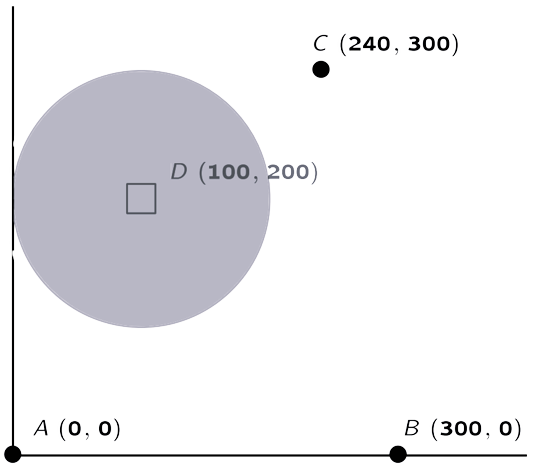
\includegraphics[width=0.4\linewidth]{images/example3.png}
        \end{figure}
        Connect them to a refinery with pipelines whose cost is proportional to the square of their length. The refinery must be at least 100 km away from point $D=(100,200)$, but 
        the oil pipelines can cross the corresponding forbidden zone. Give a mathematical model to decide where to locate the refinery to minimize the total pipeline cost. 
        \begin{itemize}
            \item Decision variables: the coordinates of the refinery $x_1,x_2$. 
            \item Objective function: we need to minimize the cost, so we have: 
            \begin{align*}
                \min{z} &=\left[ (x_1-0)^2+(x_2-0)^2 \right] \\
                        &+ \left[ (x_1-300)^2+(x_2-0)^2 \right] \\
                        &+ \left[ (x_1-240)^2+(x_2-300)^2 \right] 
            \end{align*}
            \item Constraints: there is a constraint on the location that is
                \[\sqrt{{\left( x_1-100 \right)}^2+{\left( x_2-100 \right)}^2} \geq 100\]
            \item Variable type: $x_1,x_2 \in \mathbb{R}$
        \end{itemize}
    \end{example}

    \section{Mathematical programming problem}
    The decision-making problems can be classified as: 
    \begin{itemize}
        \item Mathematical programming: one decision maker and one objective. 
        \item Multi-objective programming: one decision maker and several objectives.
        \item Stochastic programming: uncertainty level greater than zero. 
        \item Game theory: several decision makers. 
    \end{itemize}
    We will analyze the mathematical programming problems, so we have a single decision maker and a single objective.
    The optimization usually requires to minimizing or maximizing a given function. 
    Note that maximizing $f(x)$ is the same problem of minimizing $-f(x)$. The problems are characterized by: 
    \begin{itemize}
        \item Decision variables $x \in \mathbb{R}^n$: numerical variables whose values identify a solution of the problem. 
        \item Feasible region $X \subseteq \mathbb{R}^n$: distinguish between feasible and infeasible solutions.
        \item Objective function $f:X \rightarrow\mathbb{R}$: expresses in quantitative terms the value of each feasible solution. 
    \end{itemize}
    Solving a mathematical programming problem consists in finding a feasible solution which is globally optimum. It may happen that: the problem is infeasible, unbounded, has a single 
    optimal solution or has numerous optimal solutions. 
    When the problem is very hard we must settle for a feasible solution that is a local optimum. AN optimization problem can have many local optima. 
    Mathematical programming can be classified in three main categories:
    \begin{enumerate}
        \item Linear Programming.
        \item Integer Linear Programming.
        \item Nonlinear Programming. 
    \end{enumerate}
    Multi-objective programming can be taken into account in different ways. Suppose we wish to minimize $f_1(x)$ and maximize $f_2(x)$, we can: 
    \begin{enumerate}
        \item Turn it into a single objective problem by expressing the two objectives in terms of the same unit: 
            \[\min{\lambda_1f_1(x)-\lambda_2f_2(x)}\]
            for appropriate scalars $\lambda_1$ and $\lambda_2$.
        \item Optimize the primary objective function and turn the other objective into a constraint: 
            \[\max_{x \in X}f_2(x) \:\:\:\: f_1(x)\leq \epsilon\]
            for an appropriate constant $\epsilon$. 
    \end{enumerate}

\newpage

\chapter{Algorithms}
    \section{Complexity}
    \begin{definition}
        An \emph{algorithm} for a problem is a sequence of instructions that allows to solve any of its instances.
    \end{definition}
    The execution time of an algorithm depends on the instance and on the computer. We want to evaluate the complexity of the algorithm as a function of the size of the instance
    independently of the hardware. Thus, we consider the number of elementary operations and assume all have the same cost. Since it is usually hard to determine the exact number of
    elementary operations, so we consider the asymptotic number of elementary operations in the worst case. We look for a function $f(n)$ which is asymptotically an upper bound on 
    number of elementary operations needed to solve any instance of size at most $n$. 
    \begin{definition}
        A function $f$ is \emph{ordered} of $g$, written $f(n)=O(g(n))$, if $\exists c > 0$ such that $f(n) \leq cg(n)$, for $n$ sufficiently large. 
    \end{definition}
    Two classes of algorithms are distinguished according to their worst-case complexity:
    \begin{itemize}
        \item Polynomial: $O(n^d)$ for a given constant $d$.
        \item Exponential: $O(2^n)$. 
    \end{itemize}
    Algorithms with a high order polynomial complexity are not efficient in practice.
    \begin{figure}[H]
        \centering
        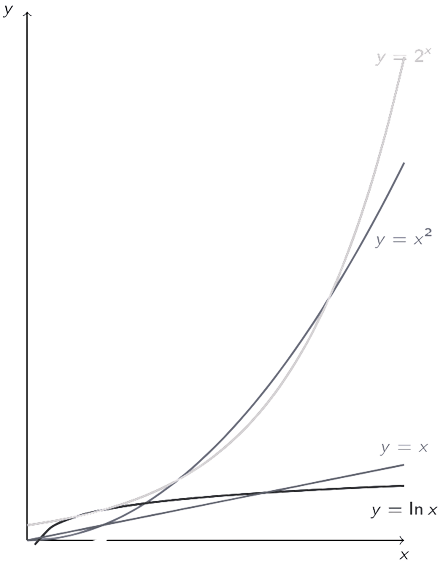
\includegraphics[width=0.25\linewidth]{images/complexity.png}
        \caption{Plot of various algorithm's complexity}
    \end{figure}

    \section{Definitions}
    \begin{definition}
        An algorithm is \emph{exact} if it provides an optimal solution for every instance. 
        
        Otherwise, it is \emph{heuristic}. 
    \end{definition}
    \begin{definition}
        A \emph{greedy algorithm} constructs a feasible solution iteratively by making at each step a locally optimal choice, without reconsidering previous choices. 
    \end{definition}





















\newpage

\chapter{Network optimization models}
    \section{Introduction}
    Many decision-making problems can be formulated in terms of graphs and networks.
    \begin{definition}
        A \emph{graph} is a pair $G=(N,E)$, with a set of nodes $N$ and a set of edges or arcs $E \subseteq N \times N$ connecting them pairwise. 
        An edge connecting the nodes $i$ and $j$ is represented by $\{i,j\}$ or $(i,j)$ if the graph is \emph{undirected} or \emph{directed} respectively. 
    \end{definition}
    \begin{example}
        A road network which connects $n$ cities can be modelled, by a graph where a city corresponds to a node, and a connection corresponds to an edge. 
        \begin{figure}[H]
            \centering
            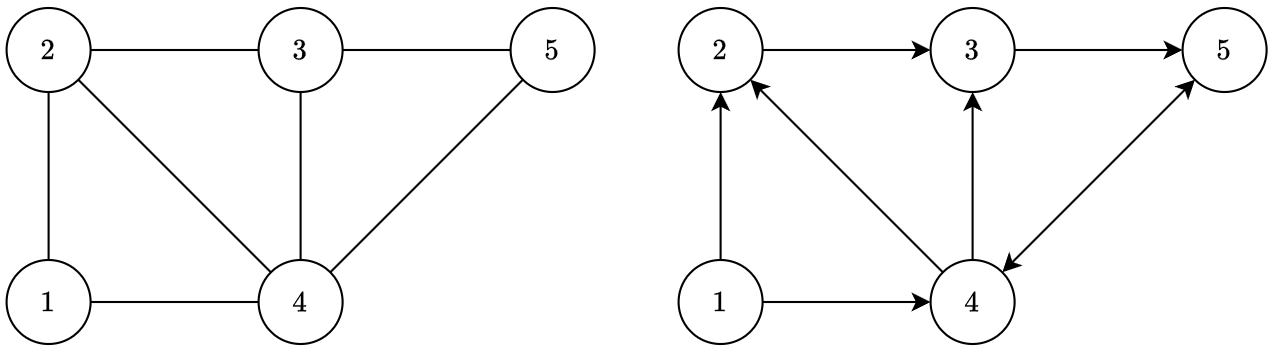
\includegraphics[width=0.75\linewidth]{images/graph.png}
        \end{figure}
        The graph on the left is undirected and defined as: 
        \begin{itemize}
            \item $N=\{1,2,3,4,5\}$
            \item $E=\{\{1,2\},\{1,4\},\{2,3\},\{2,4\},\{3,4\},\{3,5\},\{4,5\}\}$
        \end{itemize}
        The graph on the right is directed and defined as: 
        \begin{itemize}
            \item $N=\{1,2,3,4,5\}$
            \item $E^{'}=\{(1,2),(1,4),(2,3),(2,4),(3,4),(3,5),(4,5)\}$
        \end{itemize}
    \end{example}
    \begin{definition}
        Two nodes are \emph{adjacent} if they are connected by an edge. An edge $e$ is \emph{incident} in a node $v$ if $v$ is an endpoint of $e$. In undirected graphs, 
        the \emph{degree} of a node is the number of incident edges in a given node. In directed graph, the \emph{id-degree} (\emph{out-degree}) of a node is the number of arcs
        that ave it as successor (predecessor).
    \end{definition}
    \begin{example}

        In the undirected graph, we have that nodes $1$ and $2$ are adjacent and $1$ and $3$ are not. The edge $\{1,2\}$ is incident in nodes $1$ and $2$. Node $1$ has a degree $2$,
        and node $4$ has a degree of $4$. 

        In the directed graph, the node $1$ has an in-degree equal to $0$, and an out-degree equal to $2$.
        \begin{figure}[H]
            \centering
            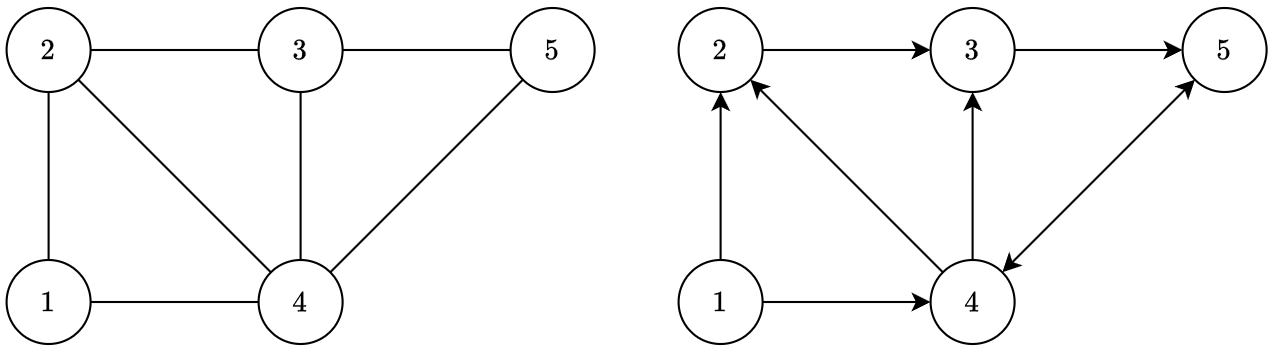
\includegraphics[width=0.75\linewidth]{images/graph.png}
        \end{figure}
    \end{example}
    \begin{definition}
        A \emph{directed path from $i \in N$ to $j \in N$} is a sequence of arcs $p=\langle \{v_1,v_2\},\{v_2,v_3\},\dots,\{v_{k-1},v_k\}\rangle $ connecting nodes $v_1$ and $v_k$. 
        Nodes $u$ and $v$ are \emph{connected} if there is a path connecting them. A graph $(N,E)$ is connected if $u,v$ are connected for any $u,v \in N$. A graph is \emph{strongly
        connected} if $u,v$ are connected by a directed path for any $u,v \in N$. A \emph{cycle} or circuit is a path with $v_1=v_k$.
    \end{definition}
    \begin{example}
        The undirected graph has a path $\langle \{2,3\},\{3,4\},\{4,5\}\rangle$ from node $2$ to node $5$. So we say those nodes are connected. 
        
        The directed graph has a directed path $\langle (3,5),(5,4),(4,2),(2,3),(3,4) \rangle$ from node $3$ to node $4$. So we say those nodes are not strongly connected. 
        
        In the undirected graph $\langle \{2,3\},\{3,5\},\{5,4\},\{4,2\}\rangle$ is a cycle. 
        In the directed graph $\langle (2,3),(3,4),(4,2) \rangle$ is a circuit. 
        \begin{figure}[H]
            \centering
            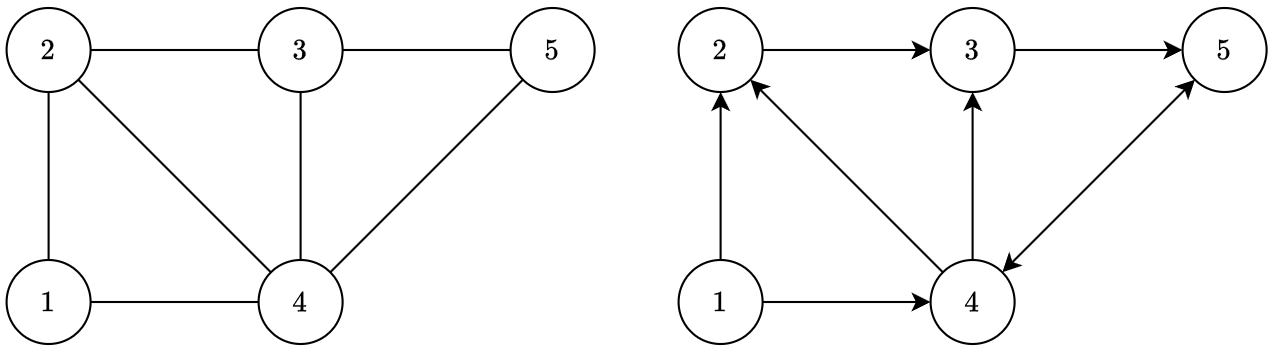
\includegraphics[width=0.75\linewidth]{images/graph.png}
        \end{figure}
    \end{example}
    \begin{definition}
        A graph is \emph{bipartite} if there is a partition $N=N_1 \cup N_2$ with $N_1 \cap N_1 = \varnothing$ such that no edge connects nodes in the same subset. 
        A graph is \emph{complete} if $E=\{ \{v_i,v_j\} | v_i,v_j \in N \land i \leq j \}$
    \end{definition}
    \begin{example}
        The graphic on the left is bipartite because we can find two subsets of nodes such that $N=N_1 \cup N_2$ with $N_1 \cap N_1 = \varnothing$ that are: $N_1=\{1,2,3\}$ and 
        $N_2=\{4,5\}$. The graph on the right is a complete graph because all the nodes are connected with each other. 
        \begin{figure}[H]
            \centering
            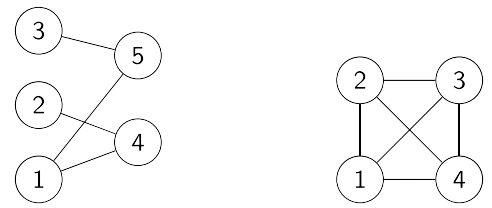
\includegraphics[width=0.5\linewidth]{images/bipcomp.png}
        \end{figure}
    \end{example}
    \begin{definition}
        Given a directed graph $G=(N,A)$ and $S \subset NM$, the \emph{outgoing cut} induced by $S$ is:
        \[ \delta^{+}(S)=\{(u,v) \in A | u \in S \land v \in N-S \} \]
        while the \emph{incoming cut} induced by $S$ is:
        \[ \delta^{-}(S)=\{(u,v) \in A | v \in S \land u \in N-S \} \]
    \end{definition}
    \begin{example}
        In the following graph we can note that: 
        \begin{itemize}
            \item $\delta^{+}(\{1,4\})=\{(1,2),(4,2),(4,5)\}$
            \item $\delta^{-}(\{1,4\})=\{(3,4),(5,4)\}$
        \end{itemize}
        \begin{figure}[H]
            \centering
            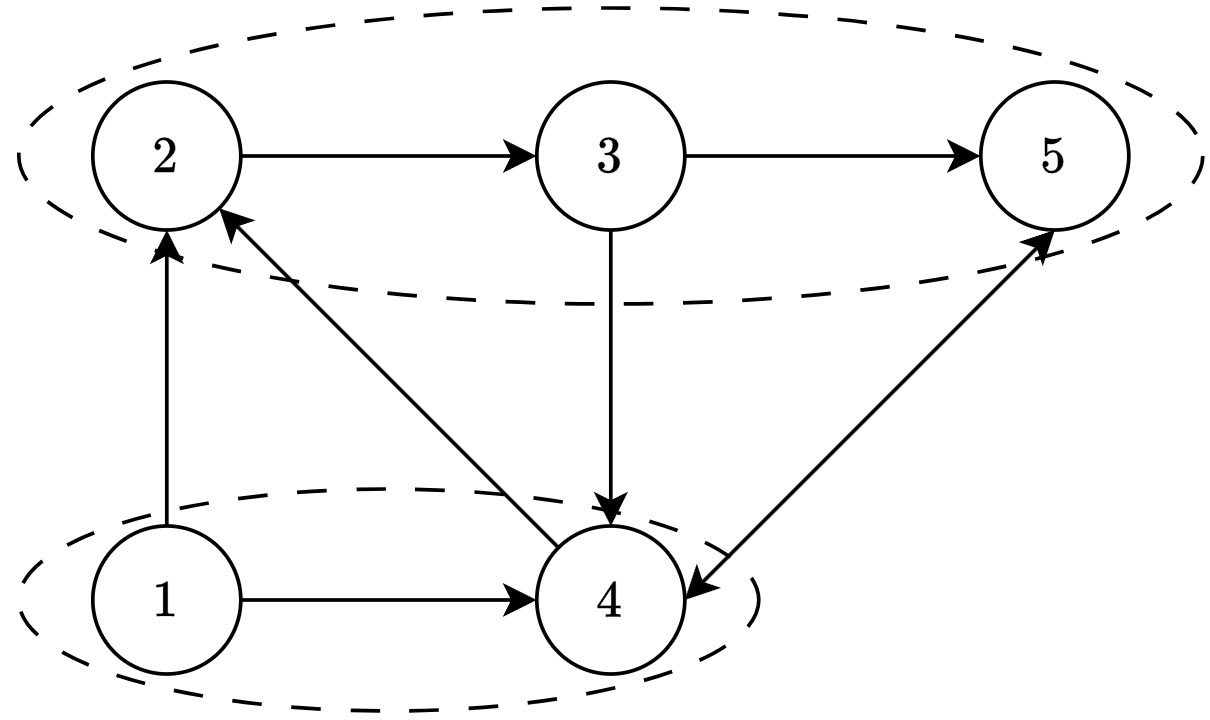
\includegraphics[width=0.75\linewidth]{images/cuts.png}
        \end{figure}
    \end{example}
    An undirected graph with $n$ nodes has at most $m=n(n-1)$ arcs. 
    A directed graph with $n$ nodes has at most $m=\dfrac{n(n-1)}{2}$ arcs.
    \begin{definition}
        A graph is said to be \emph{dense} if: 
        \[m \approx n^2\]
        and \emph{sparse} if: 
        \[m \ll n^2\]
    \end{definition}
    The best way to represent a dense graph is by using an $n \times n$ adjacency matrix, that is defined in the following way: 
    \[
    \begin{cases}
        a_{ij}=1 \:\:\:\:\:\: \textnormal{if}\:(i,j) \in A \\
        a_{ij}=0 \:\:\:\:\:\: \textnormal{otherwise}    
    \end{cases}    
    \]
    The best way to represent a sparse graph is by using lists of successors for each node. 
    \begin{example}
        The adjacency matrix for the following graph is: 
        \[A=
        \begin{bmatrix}
            0 & 1 & 0 & 1 & 0 \\
            0 & 0 & 1 & 0 & 0 \\
            0 & 0 & 0 & 1 & 1 \\
            0 & 1 & 0 & 0 & 1 \\
            0 & 0 & 0 & 1 & 0 
            \end{bmatrix}
        \]
        And the list of successor is: 
        \[S(1)=\{2,4\} \:\:\: S(2)=\{3\} \:\:\:S(3)=\{4,5\} \:\:\: S(4)=\{2,5\} \:\:\: S(5)=\{4\} \:\:\:\]
        \begin{figure}[H]
            \centering
            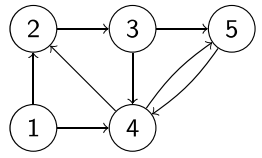
\includegraphics[width=0.3\linewidth]{images/graphs.png}
        \end{figure}
    \end{example}
    \begin{definition}
        $G^{'}=(N^{'},E^{'})$ is a \emph{sub-graph} of $G=(N,E)$ if $N^{'} \subseteq N$ and $E^{'} \subseteq E$. 
        A \emph{tree} $G_T=(N^{'},T)$ \emph{of $G$} is a connected and acyclic sub-graph of $G$. 
        $G_T=(N^{'},T)$ is a \emph{spanning tree of $G$} if it contains all nodes in $G$. 
        The \emph{leaves} of a tree are the nodes of degree one. 
    \end{definition}
    \begin{example}
        Given the following graph: 
        \begin{figure}[H]
            \centering
            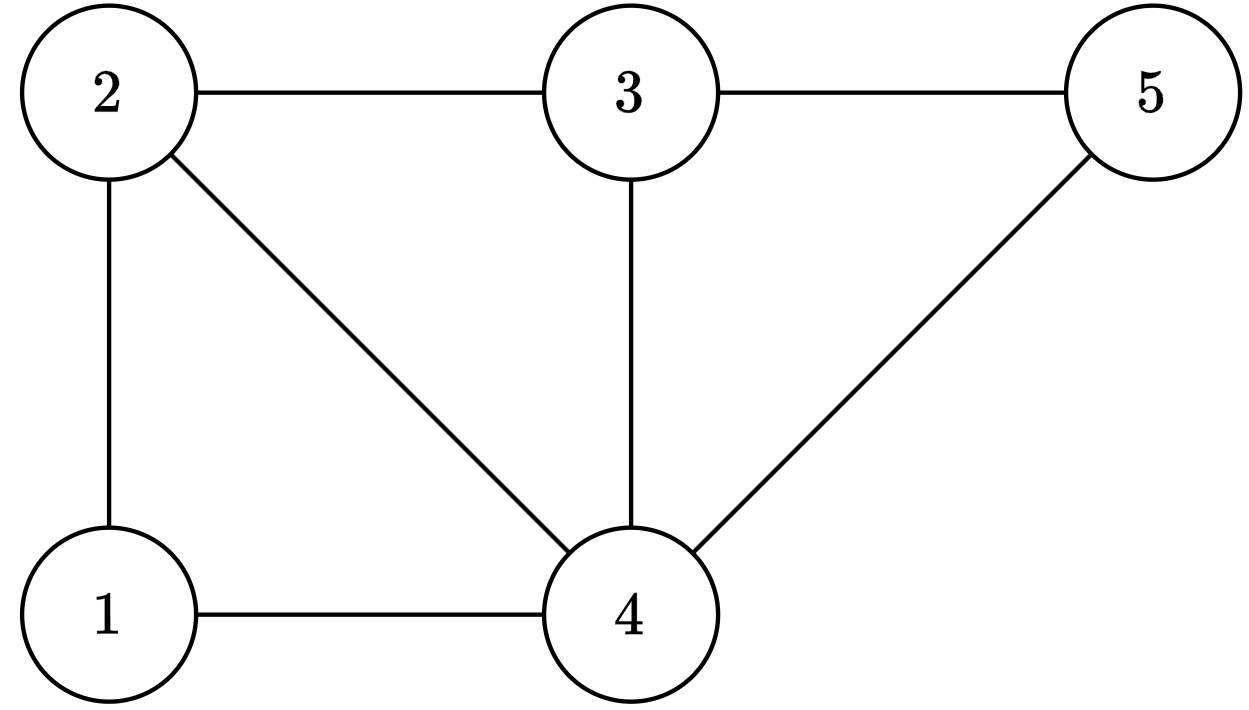
\includegraphics[width=0.3\linewidth]{images/sgraph.png}
        \end{figure}
        We can obtain respectively: a sub-graph, a tree (that is also a sub-graph), and a spanning tree in those ways: 
        \begin{figure}[H]
            \centering
            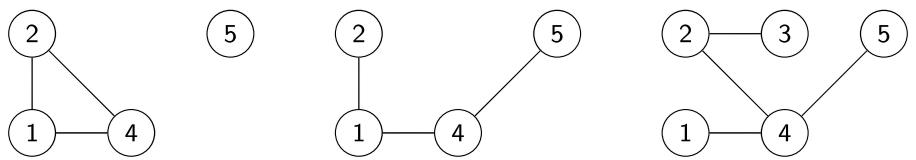
\includegraphics[width=0.8\linewidth]{images/sgraphmod.png}
        \end{figure}
    \end{example}
    The trees have the following properties: 
    \begin{enumerate}
        \item Every tree with $n$ nodes has $n-1$ edges. 
        \item Any pair of nodes in a tree is connected via a unique path. 
        \item By adding a new edge to a tree, we create a unique cycle. 
        \item Let $G_T=(N,T)$ be a spanning tree of $G=(N,E)$. Consider an edge $e \notin T$ and the unique cycle $C$ of $T \cup \{e\}$. For each edge $f \in C-\{e\}$, the 
            sub-graph $T\cup \{e\}-\{f\}$ is also a spanning tree of $G$. 
        \item Let $F$ be a partial tree contained in an optimal tree of $G$. Consider $e\{u,v\}\in \delta(S)$ of minimum cost, then there exists a minimum cost spanning tree of 
            $G$ containing $e$. 
    \end{enumerate}
    \begin{proof}[Property one]
        We will demonstrate this property with a proof by induction. For the base case we have that the claim holds for $n=1$ (tree with one node and zero edges). 
        For the inductive step we have to show that, if this is true for trees with $n$ nodes, then it is also true for those with $n+1$ nodes. 
        Let $T_1$ be a tree with $n+1$ nodes and recall that any tree with $n \geq 2$ nodes has at least two leaves. By deleting one of the leaf and its incident edge we obtain
        a tree $T_2$ with $n$ nodes. By induction hypothesis, $T_2$ has $n-1$ edges. Therefore, the tree $T_1$ has $n-1+1=n$ edges. 
    \end{proof}
    \begin{proof}[Property five]
        By contradiction, assume $T^{*} \subseteq E$ is a minimum cost spanning tree with $F \subseteq T^{*}$ and $e \notin T^{*}$. Adding edge $e$ to $T^{*}$ creates the cycle
        $C$. Let $f \in \delta(S) \cap C$: 
        \begin{itemize}
            \item If $c_e=c_f$, then $T^{*}\cup\{e\}-\{f\}$ is also optimal since it has same cost of $T^{*}$.
            \item If $c_e<c_f$, then $c\left(T^{*}\cup\{e\}-\{f\}\right)<C(T^{*})$, hence $T^{*}$ is not optimal.
        \end{itemize}
    \end{proof}

    \section{Graph reachability problem}
    Given the directed graph $G=(N,A)$ and a node $s$, determine all the nodes that are reachable from $s$. 
    \begin{algorithm}[H]
        \caption{Graph reachability problem}
            \begin{algorithmic}[1]
                \State $Q \leftarrow \{s\}$
                \State $M \leftarrow \{\varnothing\}$
                \While {$Q \neq 0$}
                    \State $u \leftarrow \textnormal{node in } Q$
                    \State $Q \leftarrow Q-\{u\}$
                    \State $M \leftarrow M \cup \{u\}$
                    \For {$(u,v) \in \delta^{+}(u)$}
                        \If {$v \notin M$ and $v \notin Q$}
                            \State $Q \leftarrow Q \cup \{v\}$
                        \EndIf
                    \EndFor
                \EndWhile
            \end{algorithmic}
    \end{algorithm}
    The worst case complexity of the previous algorithm is $O(n^2)$.
    \begin{example}
        Given the following graph and $s=2$ the algorithm makes the following steps: 
        \begin{enumerate}
            \item $Q=\{2\} \:\:\:\:\:\: M=\varnothing$
            \item $Q=\{3\} \:\:\:\:\:\: M=\{2\}$
            \item $Q=\{4,5\} \:\:\:\:\:\: M=\{2,3\}$
            \item $Q=\{5\} \:\:\:\:\:\: M=\{2,3,4\}$
            \item $Q=\varnothing \:\:\:\:\:\: M=\{2,3,4,5\}$
        \end{enumerate}
        So the nodes $\{2,3,4,5\}$ are reachable from node $2$. 
        \begin{figure}[H]
            \centering
            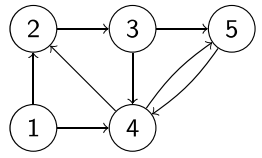
\includegraphics[width=0.3\linewidth]{images/graphs.png}
        \end{figure}
    \end{example}

    \section{Minimum spanning tree problem}
    Given an undirected graph $G=(N,E)$ and a cost function, find a spanning tree $G_T=(N,T)$ of minimum total cost: 
    \[\min_{T \in X} \sum_{e \in T}c_e\]
    where $X$ is the set of all spanning trees of $G$. 
    \begin{theorem}[Cayley - 1889]
        A complete graph with $n$ nodes $(n \geq 1)$ has $n^{(n-2)}$ spanning trees. 
    \end{theorem}
    To find the spanning tree with the minimum total cost we can use an algorithm that iteratively builds the spanning tree. The algorithm for the minimum spanning tree problem
    is the following: 
    \begin{enumerate}
        \item Select any node arbitrarily, and connect it to the nearest distinct node.
        \item Identify the unconnected node that is closest to a connected node, and then connect these two nodes. Repeat this step until all nodes have been connected.
    \end{enumerate}
    \begin{example}
        Apply the Prim's algorithm to the following graph: 
        \begin{figure}[H]
            \centering
            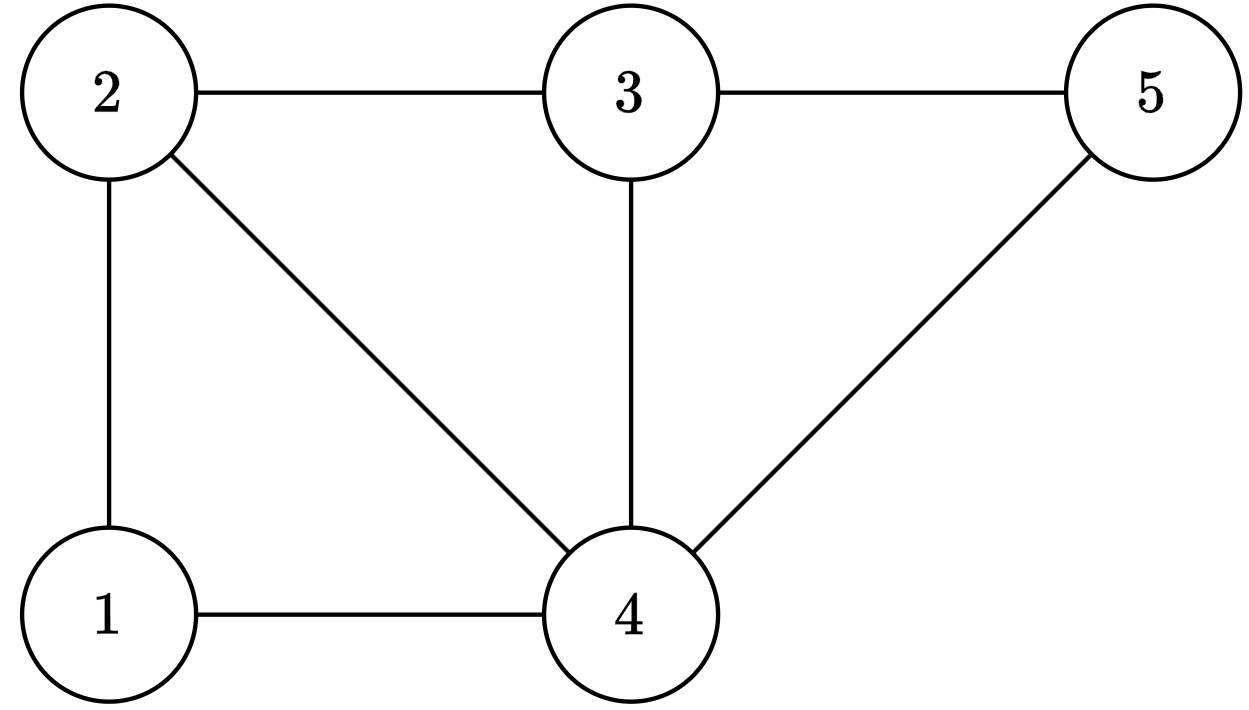
\includegraphics[width=0.3\linewidth]{images/sgraph.png}
        \end{figure}
        We select the node $3$ as starting node, and so we have $S=\{3\} \: T=\{\varnothing\}$, then:
        \begin{itemize}
            \item The edge with minimum cost is the one that connects the nodes $3$ and $4$. Now we have: $S=\{3,4\}$ and $T=\{\{3,4\}\}$.
            \item The edge with minimum cost is the one that connects the nodes $1$ and $4$. Now we have: $S=\{1,3,4\}$ and $T=\{\{3,4\},\{1,4\}\}$.
            \item The edge with minimum cost is the one that connects the nodes $4$ and $5$. Now we have: $S=\{1,3,4,5\}$ and $T=\{\{3,4\},\{1,4\},\{4,5\}\}$.
            \item The edge with minimum cost is the one that connects the nodes $4$ and $5$. Now we have: $S=N$ and $T=\{\{3,4\},\{1,4\},\{4,5\},\{2,4\}\}$.
        \end{itemize}
        The total cost in this case is equal to $c(T)=6$. Graphically, we have the following graphs: 
        \begin{figure}[H]
            \centering
            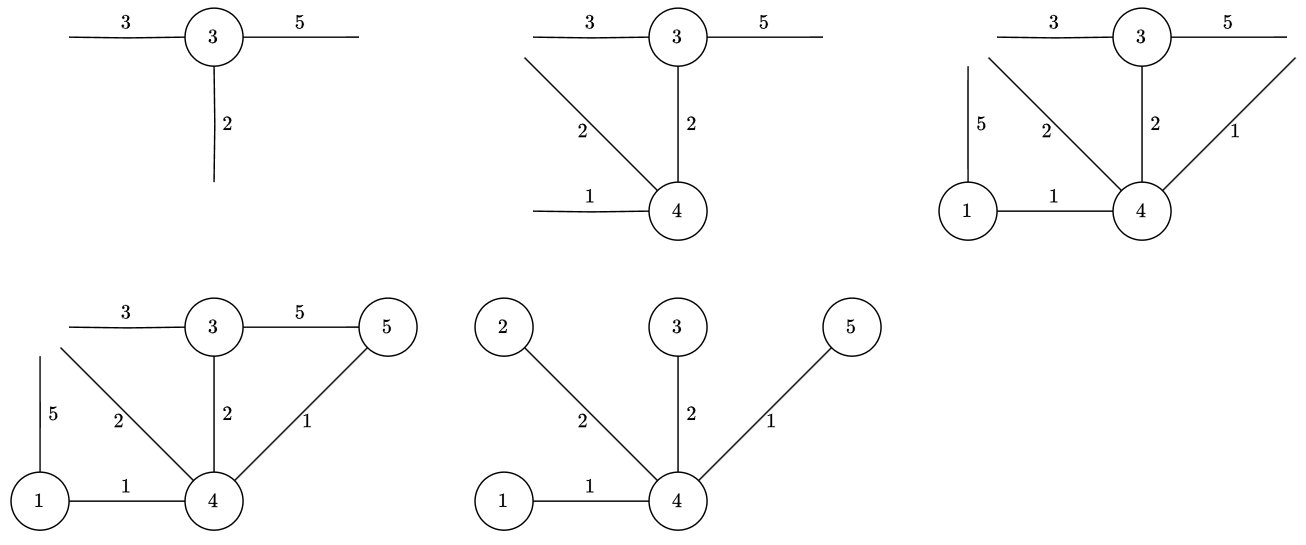
\includegraphics[width=0.75\linewidth]{images/MST.png}
        \end{figure}
    \end{example}
    Given a connected graph $G=(N,E)$ with edge cost the algorithm outputs $T \subseteq N$ of edges of $G$ such that $G_T=(N,T)$ is a minimum cost spanning tree of $G$. 
    \begin{algorithm}[H]
        \caption{Prim's algorithm for the minimum cost spanning tree problem}
            \begin{algorithmic}[1]
                \State $S \leftarrow \{u\}$
                \State $T \leftarrow \{\varnothing\}$
                \While {$\left\lvert T \right\rvert < n-1$}
                    \State $\{u,v\}\leftarrow \textnormal{edge in} \delta(S) \textnormal{of minimum cost}$
                    \State $S \leftarrow S \cup \{v\}$
                    \State $T \leftarrow T \cup \{u,v\}$
                \EndWhile
            \end{algorithmic}
    \end{algorithm}
    where $u \in S$ and $v \in N-S$. The worst-case complexity is $O(n^2)$. 
    \begin{example}[Proposition]
        Prim's algorithm is exact. 
    \end{example}        
    The exactness does not depend on the choice of the first node nor on the selected edge of minimum cost in $\delta(S)$. 
    \begin{example}[Proposition]
        Prim's algorithm is greedy. 
    \end{example}     
    At each step a minimum cost edge is selected among those in the cut $\delta (S)$ induced by the current set of nodes $S$. 
    \begin{definition}
        Given a spanning tree $T$, an edge $e \notin T$ is \emph{cost decreasing} if when $e$ is added to $T$ it creates a cycle $C$ with $C \subseteq T \cup \{e\}$ and 
        $\exists f \in C-\{e\}$ such that $c_e<c_f$. 
    \end{definition}
    \begin{example}
        Given the following graph
        \begin{figure}[H]
            \centering
            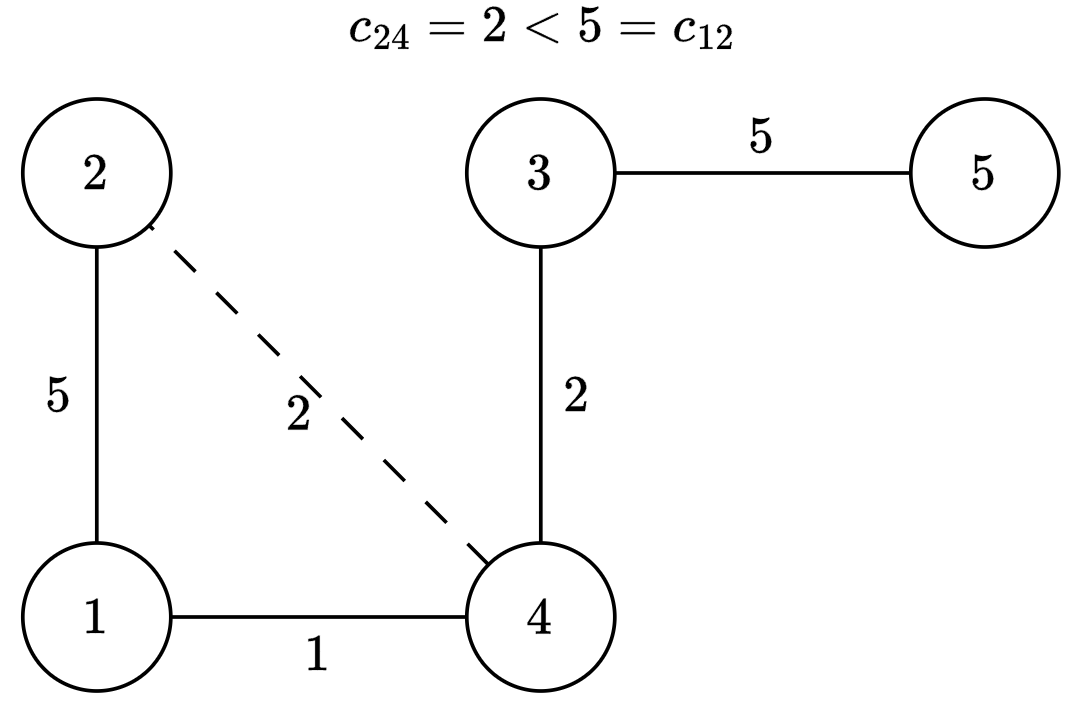
\includegraphics[width=0.5\linewidth]{images/costdecreasing.png}
        \end{figure}
        Because $c(T \cup \{e\}-\{f\})=c(T)+c_e-c_f$, if $e$ is cost decreasing, then
        \[c(T \cup \{e\}-\{f\})<c(T)\]
    \end{example}
    \begin{theorem}[Tree optimaility condition]
        A tree $T$ is of minimum total cost if and only if no cost decreasing edge exists. 
    \end{theorem}
    \begin{proof}[of direct implication]
        If a cost-decreasing edge exists, then T is not of minimum total cost.
    \end{proof}
    \begin{proof}[of inverse implication]
        If no cost-decreasing edge exists, then $T$ is of minimum total cost. Let $T^{*}$ be a minimum cost spanning tree found by Prim's algorithm. It can be verified that, by 
        exchanging one edge at a time, $T^{*}$ can be iteratively transformed into $T$ without modifying the total cost. Thus, $T$ is also optimal. 
    \end{proof}
    The optimality condition allows us to verify whether a spanning tree $T$ is optimal: it is sufficient to check that each $e \in E-T$ is not a cost-decreasing edge. 

\end{document}